\documentclass[t]{beamer}
\usetheme[darktitle]{UniversityOfManchester}

% Document properties
\title{On-SpiNNaker routing table minimisation}
\author{Andrew Mundy}

% Switch out the fonts
\usepackage{sourcesanspro}
\usepackage{sourcecodepro}

% In-presentation diagram styling
\usepackage{cancel}
\usetikzlibrary{chains, positioning}
\tikzset{
  subtable/.style = {draw, ultra thick, inner sep=0, minimum width=4em},
}

\begin{document}
\maketitle

\begin{frame}{Benchmarks}
  
\end{frame}

\begin{frame}[plain]{}
  \begin{center}
    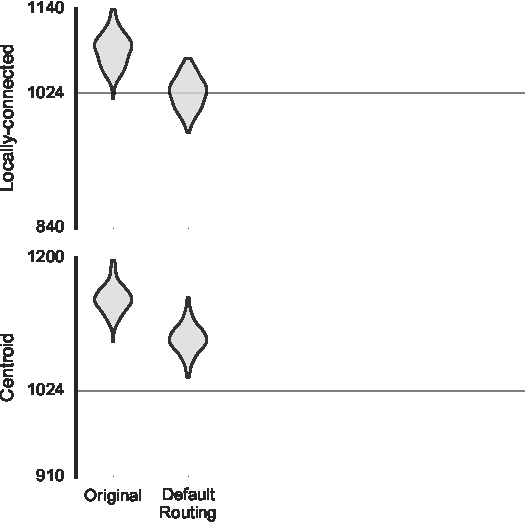
\includegraphics[page=1]{../experiments/presentation_plots}
  \end{center}
\end{frame}

\begin{frame}{Minimisation with Espresso}  % Explanation
  \begin{columns}[T]
    \begin{column}{.5\textwidth}
      \begin{itemize}
        \item Break into subtables with the same route
        \item Minimise each subtable exactly
      \end{itemize}\vskip\baselineskip

      \textbf{Exact?}

      \texttt{0000} and \texttt{0001} $\rightarrow$ \texttt{000X}

      {\color{red} \texttt{0001} and \texttt{0010} $\rightarrow$ \cancel{\texttt{00XX}}}
    \end{column}
    \begin{column}{.5\textwidth}
      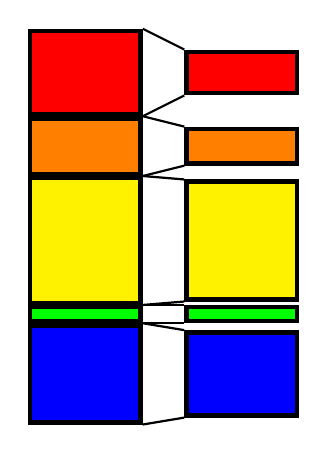
\begin{tikzpicture}[start chain=1 going below, node distance=0]
        % Diagram mostly of the form
        % A --> minimise exact --> a
        \foreach \X/\s/\t/\c in {
          A/3.0em/1.5em/red,
          B/2.0em/1.25em/orange,
          C/4.5em/4.25em/yellow,
          D/0.5em/0.50em/green,
          E/3.5em/3.00em/blue%
        }{
          \node (big\X) [subtable, minimum height=\s, fill=\c, on chain=1] {};
          \node (small\X) [subtable, minimum height=\t, fill=\c, right=1.5em of big\X] {};

          \draw [thick] (big\X.north east) -- (small\X.north west);
          \draw [thick] (big\X.south east) -- (small\X.south west);
        }
      \end{tikzpicture}
    \end{column}
  \end{columns}
\end{frame}

\begin{frame}[plain]{}
  \begin{center}
    \includegraphics[page=2]{../experiments/presentation_plots}
  \end{center}
\end{frame}

\begin{frame}{Minimisation with Espresso}
  \begin{itemize}
    \item Good when coarse routing decisions can be made with few bits
      \begin{itemize}
        \item Source-based routing doesn't allow this
      \end{itemize}
    \item Ignores the prioritization of the TCAM
  \end{itemize}
\end{frame}

\begin{frame}{Order-exploiting minimisation}  % With Espresso, explanation
  \begin{columns}[T]
    \begin{column}{.5\textwidth}
      \begin{itemize}
        \item Break into subtables with the same route
        \item \textbf{Sort in order of subtable size}
        \item Minimise each subtable \textbf{to avoid collisions with lower subtables}
      \end{itemize}\vskip.5\baselineskip

      \texttt{0001} and \texttt{0010} $\rightarrow$ \texttt{00XX} \emph{allowed} iff. no lower table contains \texttt{0000} or \texttt{0011}
    \end{column}
    \begin{column}{.5\textwidth}
      \only<1>{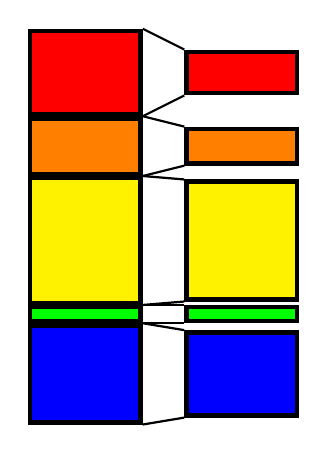
\begin{tikzpicture}[start chain=1 going below, node distance=0]
        % Diagram mostly of the form
        % A --> minimise exact --> a
        \foreach \X/\s/\t/\c in {
          A/3.0em/1.5em/red,
          B/2.0em/1.25em/orange,
          C/4.5em/4.25em/yellow,
          D/0.5em/0.50em/green,
          E/3.5em/3.00em/blue%
        }{
          \node (big\X) [subtable, minimum height=\s, fill=\c, on chain=1] {};
          \node (small\X) [subtable, minimum height=\t, fill=\c, right=1.5em of big\X] {};

          \draw [thick] (big\X.north east) -- (small\X.north west);
          \draw [thick] (big\X.south east) -- (small\X.south west);
        }
      \end{tikzpicture}}
      \only<2>{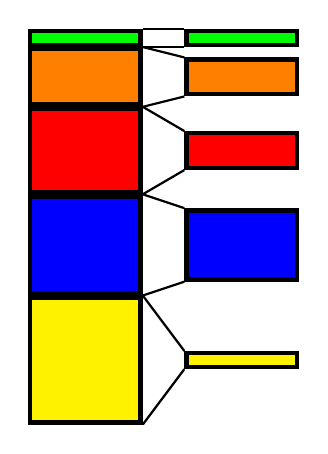
\begin{tikzpicture}[start chain=1 going below, node distance=0]
        % Same as before, but reordered according to original size
        \foreach \X/\s/\t/\c in {
          D/0.5em/0.50em/green,
          B/2.0em/1.25em/orange,
          A/3.0em/1.25em/red,
          E/3.5em/2.50em/blue,
          C/4.5em/0.50em/yellow%
        }{
          \node (big\X) [subtable, minimum height=\s, fill=\c, on chain=1] {};
          \node (small\X) [subtable, minimum height=\t, fill=\c, right=1.5em of big\X] {};

          \draw [thick] (big\X.north east) -- (small\X.north west);
          \draw [thick] (big\X.south east) -- (small\X.south west);
        }
      \end{tikzpicture}}
    \end{column}
  \end{columns}
\end{frame}

\begin{frame}[plain]{}
  \begin{center}
    \includegraphics[page=3]{../experiments/presentation_plots}
  \end{center}
\end{frame}

\begin{frame}{On-chip routing table minimisation}  % Why?
  % Timing results from Espresso, assume naive scaling
\end{frame}

\begin{frame}[plain]{}
  \begin{center}
    \includegraphics[page=4]{../experiments/presentation_plots}
  \end{center}
\end{frame}

\begin{frame}{Ordered-Covering}

\end{frame}

\begin{frame}{\emph{Up-check} rule}
  \begin{center}
    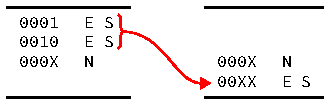
\includegraphics{../figures/rule2a_example}
  \end{center}
\end{frame}

\begin{frame}{\emph{Down-check} rule}
  \begin{center}
    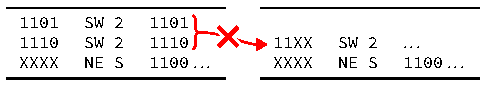
\includegraphics{../figures/rule2b_example}
  \end{center}
\end{frame}

\begin{frame}{Resolving the \emph{up-check}}
  \includegraphics<1>{../figures/upcheck_resolve_example_1}
  \includegraphics<2>{../figures/upcheck_resolve_example_2}
\end{frame}

\begin{frame}{Resolving the \emph{down-check}}
  \begin{center}
    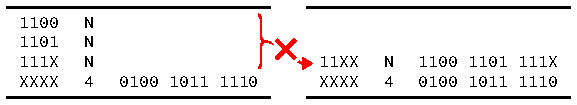
\includegraphics{../figures/downcheck_resolve_example_1}
  \end{center}
\end{frame}

\begin{frame}[plain]{}
  \begin{center}
    \includegraphics[page=5]{../experiments/presentation_plots}
  \end{center}
\end{frame}

\begin{frame}{On-chip memory usage}
  
\end{frame}

\begin{frame}{Timing}
  
\end{frame}

\begin{darkframes}
  \begin{frame}{}
    \vfill
    \begin{center}
      {\huge Thank You}\\\vskip\baselineskip
      {\Large Any questions?}
    \end{center}
    \vfill
  \end{frame}
\end{darkframes}
\end{document}
